\clearpage
\section[HKO Local Maximality]{Local maximality of the HKO pentagon product}
\label{sec:hko-local-maximum}
Let $P$ be the regular pentagon of circumradius one, centred at the origin
and with vertex $(1,0)$. In coordinates $(q_1,q_2,p_1,p_2)$ put
$K_0=P\times R(-\pi/2)P$, with symplectic form
$\omega_0=\sum_j dq_j\wedge dp_j$.
The Haim--Kislev--Ostrover capacity formula~\cite{HaimKislevOstrover2024} for this body gives
\[
 c_{\rm EHZ}(K_0)=2\cos(\pi/10)(1+\cos(\pi/5)),\qquad
 \operatorname{sys}(K_0)=\frac{3+\sqrt5}{5}>1.
\]
Here $\operatorname{sys}(K)=c_{\rm EHZ}(K)^2/(2\operatorname{vol}_4 K)$.
The counterexample itself is due to Haim--Kislev and Ostrover; the result
proved here concerns its local maximality when the number of facets stays ten.
\begin{theorem}\label{thm:hko-ten-facet-local-maximum}
There is a Hausdorff neighborhood $\mathcal U$ of $K_0$ among convex
four-dimensional polytopes with exactly ten facets such that
$\operatorname{sys}(K)\leq\operatorname{sys}(K_0)$ for $K\in\mathcal U$.
Equality holds precisely for those bodies in $\mathcal U$ obtained from
$K_0$ by translation, positive dilation and a linear symplectic map.
\end{theorem}
\subsection{The proof strategy}
The ten supporting hyperplanes may move in all four coordinate directions,
so the nearby bodies include polytopes that are no longer products.
Write
\[
 K(a)=\{x\in\mathbb R^4:a_i\cdot x\leq1,\ i=1,\ldots,10\},
 \qquad a=(a_1,\ldots,a_{10}),
\]
and let $a_0$ be the row list of $K_0$.

We construct twenty-six smooth upper bounds $U_j$ for the systolic ratio,
all equal to it at $a_0$. If one of these bounds decreases, the ratio
decreases with it. Different bounds handle different directions.
The proof first identifies their derivatives and the symmetry directions.
A linear-algebra lemma then gives a uniform negative slope transverse to
symmetry. Only at the end do we pass from these derivatives to a finite
neighborhood and recover the equality cases.

\subsection{Local coordinates and volume}
\begin{lemma}[A simple row neighborhood]\label{lem:hko-row-neighborhood}
There is a neighborhood $\mathcal N$ of $a_0$ in $(\mathbb R^4)^{10}$
on which $K(a)$ is bounded and simple, with the same vertex--facet
incidences as $K_0$. Every sufficiently Hausdorff-close ten-facet polytope
has a labelled presentation with $a\in\mathcal N$, and its rows tend to
$a_0$ as the body tends to $K_0$.
\end{lemma}
\begin{proof}
The origin stays in the interior under sufficiently small Hausdorff
perturbations of $K_0=K(a_0)$. One way to see this is through support
functions: $h_K(u)=\max_{x\in K}u\cdot x$. Write $B$ for the Euclidean
unit ball. If $rB\subset K_0$ and the Hausdorff distance from $K$ to $K_0$
is less than $\epsilon<r$, then
$h_K(u)\geq h_{K_0}(u)-\epsilon\geq r-\epsilon$ for every unit vector
$u$. Thus $(r-\epsilon)B\subset K$. On such a neighborhood polarity is
continuous: the radial function, the distance from zero to the boundary
along a unit direction, of $K^\circ$ is $1/h_K$ on the unit
sphere, and the common positive lower bound on $h_K$ makes these reciprocals
converge uniformly. The polars are uniformly bounded convex bodies, so this
also gives Hausdorff convergence.

The polar $K_0^\circ$ has the ten vertices $a_{0,i}$. Choose disjoint small
balls about them. Each vertex is uniquely exposed by some linear functional
$\ell_i$. For polars sufficiently close to $K_0^\circ$, every maximizer
of $\ell_i$ lies in the corresponding ball. Otherwise a convergent sequence
of maximizers outside that ball would limit to a maximizer on $K_0^\circ$
different from $a_{0,i}$. A maximizing face contains a vertex. A polytope
$K$ with exactly ten facets has a polar with exactly ten vertices; hence
there is exactly one polar vertex in each ball and none elsewhere. Labelling
these vertices $a_i$ gives
\[
 K=\{x:a_i\cdot x\leq1,\ i=1,\ldots,10\},\qquad a_i\longrightarrow a_{0,i}
 \quad\text{as }K\longrightarrow K_0.
\]

For completeness, the face structure is stable in this neighbourhood.
The base body is a product of two polygons and is simple: precisely four
facets meet at each vertex, with independent normals. Their four equations
therefore determine a smoothly varying intersection under a small change
of $a$. All the remaining inequalities have strict slack at that
intersection, so it remains a vertex with exactly those incident facets.

No new vertex can appear. The convex hull of the base normals contains a
ball about zero; the convex hull of sufficiently close normals contains a
smaller common ball. Consequently the bodies $K(a)$ are uniformly bounded.
If arbitrarily close parameters had a new vertex, choose four independent
active constraints there. There are finitely many four-element subsets,
so along a subsequence the same subset is active and the vertices converge
to a point of $K_0$ where those four constraints are equalities. Simplicity
forces them to be the incident facets of one of the original vertices.
Their intersection is the continuation already constructed, contradicting
newness. This argument also excludes a new vertex arising from a subset
whose normals are dependent at the base point; no invertibility assumption
for such a subset is needed.

The vertex--facet incidences therefore remain unchanged. In particular
each inequality still defines a facet. Conversely,
small changes of the ten normals give Hausdorff-small changes of $K(a)$:
their convex hulls converge, contain a common ball about zero, and polarity
is continuous there.

\end{proof}

\begin{lemma}[Smooth volume and its derivative]\label{lem:hko-smooth-volume}
On a sufficiently small neighborhood $\mathcal N$ as above, $V(a)=
\operatorname{vol}_4K(a)$ is smooth and positive. If $F_i(a)$ has centroid
$\bar x_i(a)$, then
\[
 DV(a)[h]=-\sum_{i=1}^{10}
 \frac{\operatorname{vol}_3(F_i(a))}{\|a_i\|}
 \langle h_i,\bar x_i(a)\rangle.
\]
\end{lemma}
\begin{proof}
The fixed incidences express each vertex smoothly in the rows. A fixed
boundary triangulation then expresses volume smoothly in those vertices.
On the moving facet, differentiating
$\langle a_i+\epsilon h_i,x(\epsilon)\rangle=1$ gives outward normal
velocity $-\langle h_i,x\rangle/\|a_i\|$. Integrating this velocity over
the facets and using their centroids gives the formula.
\end{proof}

\subsection*{The concrete base point and its volume}
Put $t=\tan(\pi/5)$, $s=(5-t^2)/2=\sqrt5$, and
\[
 t^4-10t^2+5=0,\quad 0<t<1,\qquad
 \alpha=(3-s)/2,\quad b=t(1+s)/2,\quad d=s-1.
\]
The selected root is unique in $(0,1)$: the polynomial is strictly decreasing
there and changes sign. For the circumradius-one pentagon with vertex $(1,0)$,
the edge normals have arguments $(2k+1)\pi/5$ and lengths $\sec(\pi/5)=d$.
Rotating the second factor by $-\pi/2$ gives the following ten rows $a_{0,i}$, in
$(q_1,q_2,p_1,p_2)$ order:
\[
\begin{pmatrix}
1&t&0&0\\ -\alpha&b&0&0\\-d&0&0&0\\-\alpha&-b&0&0\\1&-t&0&0\\
0&0&t&-1\\0&0&b&\alpha\\0&0&0&d\\0&0&-b&\alpha\\0&0&-t&-1
\end{pmatrix}.
\]
These rows give the normalized facet presentation of $K_0$.
Writing $\theta=\pi/5$, the area of one pentagon is the sum of five
triangles with central angle $2\theta$, hence
$B=\frac52\sin(2\theta)=5\sin\theta\cos\theta$.
Fubini therefore gives
\[
 V_0=B^2=25\sin^2\theta\cos^2\theta
 =\frac{25(5+s)}{32}=\frac{25(15-t^2)}{64}.
\]
To specialize Lemma~\ref{lem:hko-smooth-volume}, observe that $F_i$ is an edge times the other centered pentagon. Its centroid is
$\bar x_i=a_{0,i}/\|a_{0,i}\|^2$, its three-volume is $2\sin\theta\,B$,
and $\|a_{0,i}\|=\sec\theta$. Consequently
\[
 DV_0[h]=-\mu\sum_{i=1}^{10}a_{0,i}\cdot h_i,\qquad
 \mu=10\sin^2\theta\cos^4\theta=\frac{25}{32}+\frac{5s}{16}.
\]
This gives the volume derivative for every row perturbation at the base point.

\subsection{The touching upper bounds}
For an ordered facet word $\sigma=(\sigma_1,\ldots,\sigma_m)$, write
\[
 C_\sigma(a)=
 \begin{pmatrix}a_{\sigma_1}&\cdots&a_{\sigma_m}\\1&\cdots&1\end{pmatrix},
 \qquad e=(0,0,0,0,1)^T.
\]
The equations $C_\sigma(a)\beta=e$ impose closure and normalization.
For positive feasible weights let
\[
 Q_\sigma(a,\beta)=\sum_{j<i}\beta_i\beta_j
 \omega_0(a_{\sigma_j},a_{\sigma_i}),\qquad
 A_\sigma(a)=\frac1{2Q_\sigma(a,\beta(a))},\qquad
 U_\sigma(a)=\frac{A_\sigma(a)^2}{2V(a)}.
\]
When $Q_\sigma>0$, the variational capacity formula gives
$\operatorname{sys}(K(a))\leq U_\sigma(a)$.

Let $T$ be the tangent space at $a_0$ to the orbit generated by translations,
positive dilations and linear symplectic maps. The following lemma records
the finite calculation that will be used in the rest of the proof.
\begin{lemma}[Exact upper bounds and symmetry directions]\label{lem:hko-exact-bounds}
The space $T$ has dimension fifteen. On a neighborhood of $a_0$ there are
twenty-six smooth functions $U_j$ such that
\[
 \operatorname{sys}(K(a))\leq U_j(a),\qquad
 U_j(a_0)=\operatorname{sys}(K_0).
\]
Their derivative rows $r_j=DU_j(a_0)$ vanish on $T$, have rank twenty-five,
and satisfy
\[
 \sum_{j=1}^{26}\lambda_jr_j=0,\qquad
 \lambda_j>0,\qquad \sum_{j=1}^{26}\lambda_j=1.
\]
\end{lemma}
The construction and computer-algebra verification of this lemma occupy
the following calculations. Holding selected weights fixed and solving
the five closure and normalization equations for the others produces the
smooth sections: an invertible five-column minor gives smoothness, and
strict positivity at the base point persists nearby.

\subsection*{One of the twenty-six upper bounds}

We now work through one of the twenty-six upper bounds to illustrate the
construction and differentiation. The other twenty-five are constructed
in the same way. The exact computations for all twenty-six were verified
using a computer algebra system. Appendix~\ref{app:hko-cas} gives the complete
program with explanations of its checks.

% Corresponds to entry 2 (zero-based) of the computational witness.
Consider the seven-facet word and position sets
\[
 \sigma=(2,3,8,9,5,4,6),\quad I=(1,2,3,4,5),\quad J=(6,7).
\]
We solve closure and normalization for the weights at positions $I$ and
hold the weights at positions $J$ fixed. These are positions in the word,
not facet labels. Set
\[
 r=\frac{6909830056250513}{10^{17}},\quad
 c=\frac{t^2+5}{40},\quad z=\frac{5-t^2}{20}=\frac{s}{10},\quad
 k=\frac{3-t^2}{4}.
\]
Fix $\beta_6=r$ and $\beta_7=z$; the decimal-looking rational is an exact rational
choice, not a rounding assertion. The complete base vector is
\[
 \beta_0=(c+kr,\ c-r,\ c,\ c,\ z-kr,\ r,\ z)^T.
\]
At this word the closure matrix's selected minor is
\[
 M=C_\sigma(a_0)_I=
 \begin{pmatrix}
 -\alpha&-d&0&0&1\\b&0&0&0&-t\\0&0&0&-b&0\\
 0&0&d&\alpha&0\\1&1&1&1&1
 \end{pmatrix},\qquad \det M=10(1-t^2)>0.
\]
The full matrix is obtained by adjoining columns $(a_4,1)^T$ and $(a_6,1)^T$.
Writing $e=(0,0,0,0,1)^T$, define the nearby section by
\[
 \beta_J(a)=(r,z)^T,\qquad
 \beta_I(a)=C_\sigma(a)_I^{-1}\bigl(e-C_\sigma(a)_J(r,z)^T\bigr).
\]
Direct substitution gives $C_\sigma(a_0)\beta_0=e$ and $\beta_0>0$.
For example $0.726<t<0.727$ and $0.069<r<0.070$ suffice to check all
seven signs from the displayed formulas. Invertibility and positivity persist
in a neighborhood.

Use $\omega(x,y)=x_{q_1}y_{p_1}+x_{q_2}y_{p_2}-x_{p_1}y_{q_1}-x_{p_2}y_{q_2}$ and
\[
 Q_\sigma(a,\beta)=\sum_{j<i}\beta_i\beta_j\omega(a_{\sigma_j},a_{\sigma_i}).
\]
At the fixed base geometry, solving closure with arbitrary
$(\beta_6,\beta_7)=(u,v)$ gives the particularly simple identity
\[
 Q_\sigma=-4tv^2+(2t-2t^3/5)v.
\]
It is independent of $u$ and has its maximum at $v=z$; its value is $Q_0=t/5$.
Thus its Hessian on the two-dimensional closure affine space is singular
(in the $(u,v)$ coordinates it is $\operatorname{diag}(0,-8t)$).
The five-by-five closure minor is nevertheless invertible, so the displayed
feasible section continues smoothly and supplies an upper bound nearby.
\[
 A_0=\frac1{2Q_0}=\frac5{2t}=5t-\frac{t^3}{2},\qquad
 U_0=\frac{A_0^2}{2V_0}=\frac{11-t^2}{10}>1.
\]
The HKO capacity formula gives
$c_{\rm EHZ}(K(a_0))=2\cos(\pi/10)(1+\cos(\pi/5))=A_0$.
Thus the constructed upper bound agrees with the systolic ratio at the
base point.

\subsection*{A worked coordinate outside product-preserving perturbations}
We now choose a perturbation that varies the first momentum component of
the second $q$-facet's normal:
\[
 h_2=(0,0,1,0),\qquad h_i=0\quad(i\ne2).
\]
% This is flat coordinate 6 in the verifier's zero-based storage.
Put $w=c+kr=\beta_{0,1}$. Differentiated closure gives
\[
 D\beta_J[h]=0,\qquad D\beta_I[h]=-wM^{-1}(0,0,1,0,0)^T
 =w\begin{pmatrix}
 t^3/20-t/4\\t^3/20-t/4\\t^3/40-3t/8\\-3t^3/20+5t/4\\t^3/40-3t/8
 \end{pmatrix}.
\]
Inserting these values into the product rule for $Q$ gives the exact scalar
\[
 DQ[h]=\frac{3-t^2}{80}+
 \left(\frac{3t^2}{20}-\frac14\right)r
 -\frac{t^2+5}{4}r^2=:q_h.
\]
Since $a_2$ has zero momentum coordinates, $DV_0[h]=0$, while
\[
 DA[h]=-\frac{25}{2t^2}q_h,\qquad
 DU[h]=-\frac{125}{4t^3V_0}q_h.
\]
This coefficient of the upper-bound derivative is approximately
$-0.1801707325$. Changing only the two polygon factors keeps every
$q$-facet normal in the $q$-plane. This perturbation adds a $p_1$-component
to one of those normals, so the derivative describes a change of the upper
bound outside that product family.

\subsection{Computing the twenty-six derivatives}
\label{subsec:hko-local-maximum-computation-with-sagemath}
The table on page~\pageref{page:hko-exact-choices} gives the exact fixed values for every section,
including the worked entry. Except at entry 22, the minor positions are $I=(1,2,3,4,5)$ and
$J=(6,\ldots,m)$. Entry 22 instead has $I=(1,2,3,4,6)$ and $J=(5,7)$.
The table is ordered by the witness's zero-based certificate
index. For each table row set $\beta_J=u$ and compute
\[
 \beta_I=C_I^{-1}(e-C_Ju),\qquad
 (D\beta)_J[h]=0,\qquad
 (D\beta)_I[h]=-C_I^{-1}(DC[h])\beta.
\]
For each of the forty coordinate directions, compute
\begin{align*}
 DQ[h]&=\sum_{j<i}\bigl((D\beta_i[h])\beta_j+\beta_i(D\beta_j[h])\bigr)
       \omega(a_{\sigma_j},a_{\sigma_i})\\
 &\quad+\sum_{j<i}\beta_i\beta_j
 \bigl(\omega(h_{\sigma_j},a_{\sigma_i})+\omega(a_{\sigma_j},h_{\sigma_i})\bigr),\\
 R[h]&=-\frac{A_0}{2V_0Q_0^2}DQ[h]
       -\frac{A_0^2}{2V_0^2}DV_0[h].
\end{align*}
Together with the explicit table these formulas specify the entire
$26\times40$ matrix $R$ exactly.

The finite predicates are: every word has distinct valid labels;
$\det C_I\ne0$; $C\beta=e$; all $\beta_i>0$; $Q=t/5$;
the differentiated closure equations hold; the rows annihilate the fifteen
symmetry columns; $\operatorname{rank}R=25$; and the one-dimensional kernel
of $R^T$ has a vector whose entries have one strict sign. Normalize that
vector to sum to one, producing $\lambda>0$, $\lambda^TR=0$.
The symmetry columns are explicitly $h_i=-a_{i,j}a_i$ for $j=1,\ldots,4$,
$h_i=-a_i$, and $h_i=-X^Ta_i$ for the ten generators
\[
 X=\begin{pmatrix}A&B\\C&-A^T\end{pmatrix},\qquad B=B^T,\ C=C^T,
\]
using the four matrix units for $A$ and the three symmetric matrix units
for each of $B,C$. Their column rank is required to be fifteen.
These exact arithmetic checks establish the asserted independence, rank and
positive relation. The constructions above give smooth feasible sections
on a common neighborhood, and the HKO capacity formula gives the touching
identities. This proves Lemma~\ref{lem:hko-exact-bounds}.

\subsection{The transverse slope estimate}

The exact calculation is now summarized by
Lemma~\ref{lem:hko-exact-bounds}. We use only its rank and positivity
statements in the remaining argument.

\begin{lemma}[Uniformly negative transverse slopes]\label{lem:hko-negative-slopes}
Choose a linear complement $S$ to the symmetry tangent space $T$, so that
$(\mathbb R^4)^{10}=T\oplus S$ and $\dim S=25$.
There is $\eta>0$ such that
\[
 \min_{1\leq j\leq26}r_j(v)\leq-\eta\|v\|
 \qquad\text{for every }v\in S.
\]
\end{lemma}
\begin{proof}
The rows have rank twenty-five and vanish on the fifteen-dimensional
space $T$. Their common kernel is therefore exactly $T$, and their
restrictions span $S^*$.
For $v\in S\setminus\{0\}$, suppose that every $r_j(v)$ were
nonnegative. Their positively weighted sum is zero, so each would have
to vanish. Then $v\in T\cap S=\{0\}$, a contradiction.
Thus $\min_jr_j(v)<0$ for every nonzero transverse direction.

The function $v\mapsto\min_jr_j(v)$ is continuous on the unit sphere of
$S$. Its maximum there is strictly negative by compactness. Write that
maximum as $-\eta$ and use homogeneity to obtain the assertion.
\end{proof}

Figure~\ref{fig:hko-upper-mechanism} illustrates the slope condition in
one and two transverse dimensions.
\begin{figure}[htbp]
\centering
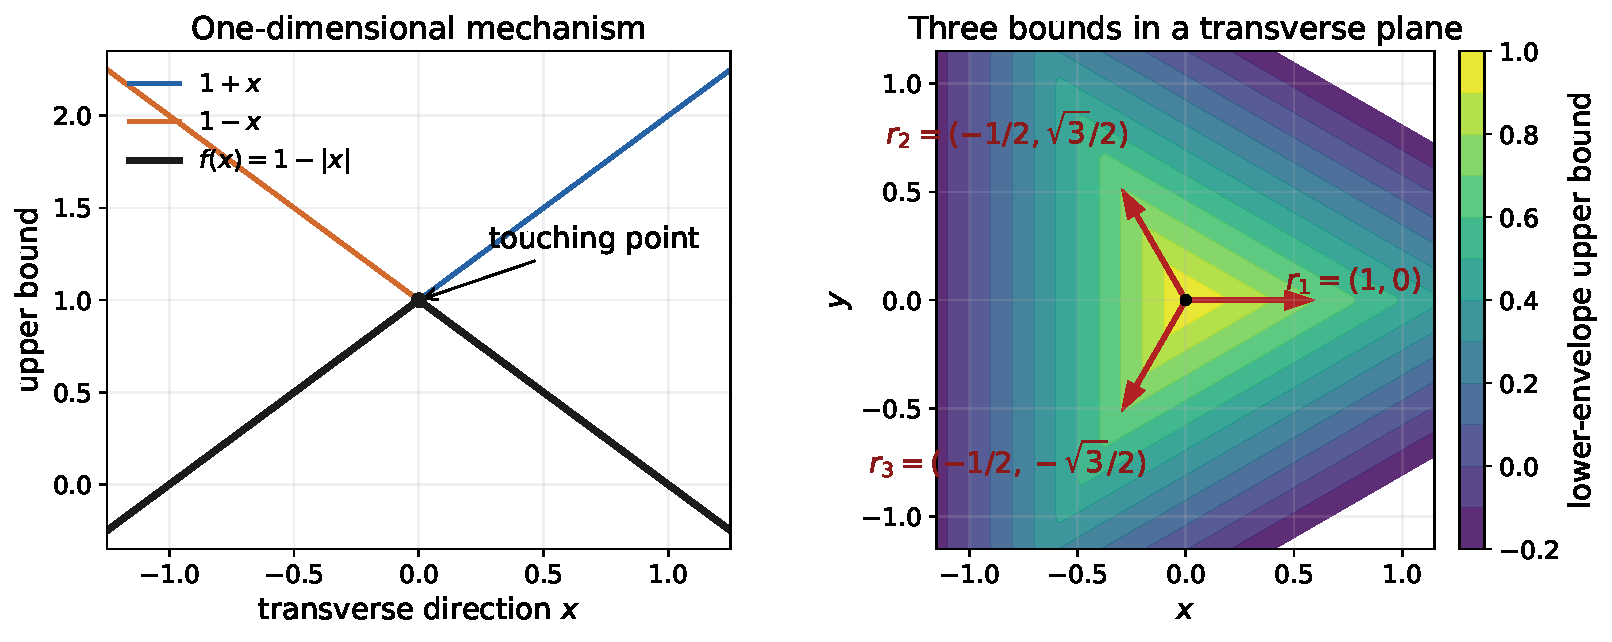
\includegraphics[width=\linewidth]{recovered/hko-figures/upper-bound-mechanisms.pdf}
\caption{Toy models of touching upper bounds. Left: the lower envelope of
$1+x$ and $1-x$ is $1-|x|$. Right: level sets of the lower envelope of
three affine functions with gradients
$(1,0)$, $(-1/2,\sqrt3/2)$ and $(-1/2,-\sqrt3/2)$.
The gradients span the plane and sum to zero, and the envelope decreases
in every nonzero direction. In the proof the systolic ratio lies below
the envelope and agrees with it at the base point.}
\label{fig:hko-upper-mechanism}
\end{figure}

\subsection{From slopes to a neighborhood}

We now pass from the derivative estimate to nearby bodies. The uniform
constant $\eta$ lets us choose one neighborhood for all transverse
directions.

\begin{lemma}[Strict decrease on the slice]\label{lem:hko-slice-decrease}
For all sufficiently small nonzero $v\in S$,
\[
 \operatorname{sys}(K(a_0+v))
 \leq\operatorname{sys}(K_0)-\frac\eta2\|v\|
 <\operatorname{sys}(K_0).
\]
\end{lemma}
\begin{proof}
There are only twenty-six smooth upper bounds. Their differentiability
at $a_0$ therefore supplies a common neighborhood in which
\[
 |U_j(a_0+v)-U_j(a_0)-r_j(v)|
 \leq\frac\eta2\|v\|\qquad(j=1,\ldots,26).
\]
Shrink it so that all bounds are defined and dominate the ratio there.
For each $v\in S$, Lemma~\ref{lem:hko-negative-slopes} supplies an index
with $r_j(v)\leq-\eta\|v\|$. Since $U_j(a_0)=\operatorname{sys}(K_0)$,
\[
 \operatorname{sys}(K(a_0+v))\leq U_j(a_0+v)
 \leq\operatorname{sys}(K_0)-\frac\eta2\|v\|.\qedhere
\]
\end{proof}

\begin{lemma}[Local symmetry decomposition]\label{lem:hko-symmetry-decomposition}
Every row list sufficiently close to $a_0$ is the image of some
$a_0+v$, with $v\in S$ small, under a symmetry close to the identity.
The symmetry and $v$ can be chosen smoothly in local group coordinates.
\end{lemma}
\begin{proof}
Translation by $y$, dilation by $\rho>0$ and a linear symplectic map $M$
act on the rows, respectively, by
\[
 a_i\mapsto\frac{a_i}{1+a_i\cdot y},\qquad
 a_i\mapsto\rho^{-1}a_i,\qquad
 a_i\mapsto M^{-T}a_i.
\]
These actions are smooth near the identity. Choose fifteen local
coordinates $\theta$ for this symmetry group and write its action as
$g(\theta)$. The map
\[
 \Phi(\theta,v)=g(\theta)\cdot(a_0+v),\qquad v\in S,
\]
has derivative at $(0,0)$ with image $T$ in the group variables and
image $S$ in the slice variables. The fifteen symmetry derivatives are
independent by Lemma~\ref{lem:hko-exact-bounds}. Thus $D\Phi(0,0)$ is
an isomorphism, and the inverse function theorem gives the decomposition.
\end{proof}

The toy model in Figure~\ref{fig:hko-symmetry-extension} shows how a
strict transverse maximum becomes a family of equal maxima along symmetry.
\begin{figure}[htbp]
\centering
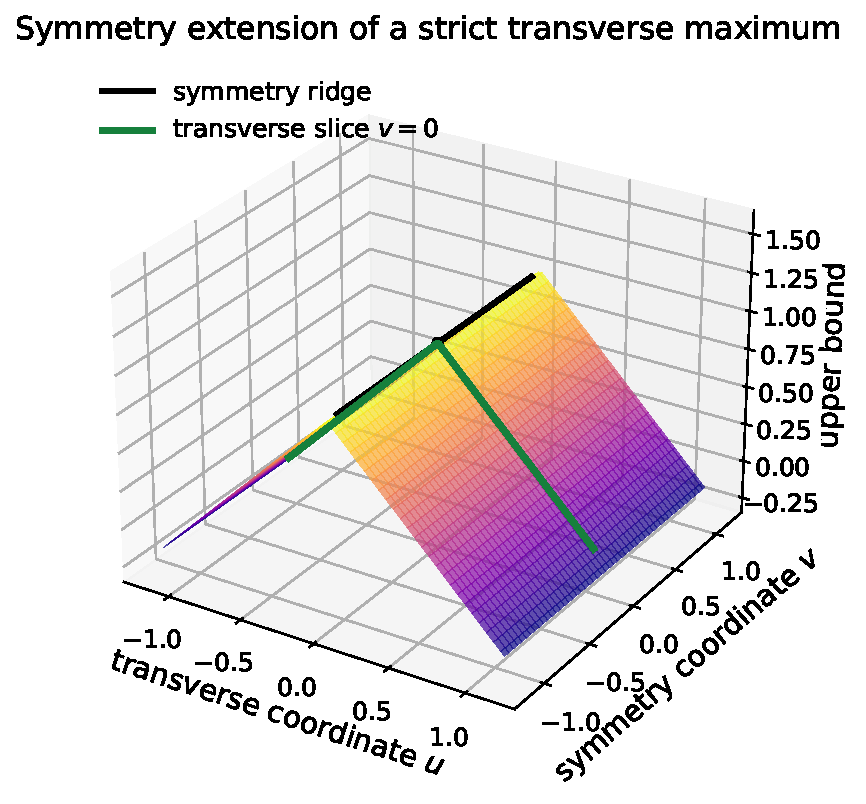
\includegraphics[width=0.72\linewidth]{recovered/hko-figures/symmetry-extension.pdf}
\caption{The toy function $f(u,v)=1-|u|$ has a strict maximum on the
transverse slice $v=0$ and is constant along the symmetry coordinate $v$.
Its maxima form the ridge $u=0$. In the HKO proof the symmetry tangent
space $T$ has dimension fifteen and the transverse space $S$ has dimension
twenty-five. The picture illustrates their roles in the local decomposition.}
\label{fig:hko-symmetry-extension}
\end{figure}

\begin{proof}[Proof of Theorem~\ref{thm:hko-ten-facet-local-maximum}]
By Lemma~\ref{lem:hko-row-neighborhood}, a sufficiently Hausdorff-close
ten-facet body has a row list in the neighborhood of
Lemma~\ref{lem:hko-symmetry-decomposition}. It is therefore a symmetry
image of $K(a_0+v)$ for some small $v\in S$. The ratio is unchanged by
that symmetry. Lemma~\ref{lem:hko-slice-decrease} gives a strict decrease
if $v\ne0$, and equality if $v=0$. Equality consequently forces the
body to be a symmetry image of $K_0$. Conversely, every such image
has the same ratio as $K_0$.
\end{proof}

\clearpage
\subsection*{The twenty-six exact choices}
\label{page:hko-exact-choices}
The constants $c=(t^2+5)/40$ and $z=(5-t^2)/20$ are as above.
Facet labels and positions start at one; entry numbers start at zero to
identify the rows in the accompanying computational witness.
Every finite decimal in the table denotes its exact rational value.
\begingroup
\small\renewcommand{\arraystretch}{1.25}
\renewcommand{\baselinestretch}{1.2}\selectfont
% All facet labels and word positions are 1-based.
\begin{longtable}{rll>{\raggedright\arraybackslash}p{0.49\textwidth}}
Entry & Word $\sigma$ & Fixed positions $J$ & Exact fixed values \\
\hline
0 & $(1,2,8,4,10,6)$ & $(6)$ & $(c)$ \\
1 & $(1,2,8,7,4,10)$ & $(6)$ & $(z)$ \\
2 & $(2,3,8,9,5,4,6)$ & $(6,7)$ & $(0.06909830056250513,z)$ \\
3 & $(1,8,7,3,4,10)$ & $(6)$ & $(z)$ \\
4 & $(2,9,8,5,4,6)$ & $(6)$ & $(z)$ \\
5 & $(2,8,4,5,6,10)$ & $(6)$ & $(c)$ \\
6 & $(1,6,2,8,5,4,10)$ & $(6,7)$ & $(0.180901699437495,c)$ \\
7 & $(1,7,8,4,3,9,10)$ & $(6,7)$ & $(0.0202254248593736825 t^{2} + 0.0584220259843842225,0.18090169943749473)$ \\
8 & $(1,5,7,6,3,10,9)$ & $(6,7)$ & $(0.020225424859373655 t^{2} + 0.058422025984384415,0.18090169943749462)$ \\
9 & $(2,8,4,3,9,5,6)$ & $(6,7)$ & $(0.1809016994374947,z)$ \\
10 & $(2,3,9,8,4,5,6)$ & $(6,7)$ & $(0.18090169943749512,z)$ \\
11 & $(2,8,9,5,7,6,3)$ & $(6,7)$ & $(0.18090169943749473,c)$ \\
12 & $(1,7,8,4,10,2)$ & $(6)$ & $(c)$ \\
13 & $(1,7,4,3,9,10)$ & $(6)$ & $(c)$ \\
14 & $(2,9,5,6,7,3)$ & $(6)$ & $(c)$ \\
15 & $(2,8,3,9,5,6)$ & $(6)$ & $(z)$ \\
16 & $(2,8,4,5,10,6)$ & $(6)$ & $(c)$ \\
17 & $(1,7,3,2,8,4,10)$ & $(6,7)$ & $(0.18090169943749507,z)$ \\
18 & $(1,5,6,7,3,2,9)$ & $(6,7)$ & $(0.06909830056250547,z)$ \\
19 & $(1,7,3,9,5,6,2)$ & $(6,7)$ & $(c,0.06909830056250552)$ \\
20 & $(1,8,5,4,6,10,2)$ & $(6,7)$ & $(c,0.14926352961534042)$ \\
21 & $(1,6,2,8,7,4,10)$ & $(6,7)$ & $(z,0.1809016994374947)$ \\
22 & $(1,5,7,4,3,9,10)$ & $(5,7)$ & $(0.18090169943749482,c)$ \\
23 & $(1,7,3,4,10,9,5)$ & $(6,7)$ & $(c,0.06909830056250518)$ \\
24 & $(1,7,6,3,10,9,5)$ & $(6,7)$ & $(0.1809016994374948,c)$ \\
25 & $(2,8,9,5,4,6,3)$ & $(6,7)$ & $(z,0.12028993467659169)$ \\
\end{longtable}


\endgroup
